\documentclass[output=paper]{langsci/langscibook} 
\ChapterDOI{10.5281/zenodo.4954481}
\author{Yannic Bracke\affiliation{Friedrich-Schiller-Universität Jena}}
\title[Namibian German and gender]{Namibian German and gender: A corpus study on the use of transferred lexical items}

\abstract{This chapter presents a quantitative corpus study of informal speech from male and female adolescent and adult Namibians with L1 German. A key feature of Namibian German is various forms of language mixing, mostly with material from English and Afrikaans. Previous sociolinguistic research, as well as statements by community members, suggest that male speakers might use more other-language material in their speech. I identified other-language material in a corpus of peer group conversations by Namibian German adolescents and adults and investigated the amount of transferred lexical items (other-language material excluding multi-word code-switches) that speakers of different age and gender used. Furthermore, I analyzed the proportion of the donor languages English and Afrikaans. Concerning the frequency of transferred lexical items, the results show an age difference between younger and older speakers, but fewer clear differences between speakers of different gender. English is the prime donor language in all groups, but subtle differences in the proportion of Afrikaans may point to interesting sociolinguistic dynamics.}
\IfFileExists{../localcommands.tex}{
  % add all extra packages you need to load to this file

\usepackage{tabularx,multicol}
\usepackage{url}
\urlstyle{same}

\usepackage{listings}
\lstset{basicstyle=\ttfamily,tabsize=2,breaklines=true}

\usepackage{langsci-optional}
\usepackage{langsci-lgr}
\usepackage{langsci-gb4e}
% \usepackage{langsci-plots}
\usepackage{pgfplots}

\usepackage{siunitx}
\sisetup{group-digits=false}

\usepackage{amssymb}% http://ctan.org/pkg/amssymb
\usepackage{pifont}% http://ctan.org/pkg/pifont
\newcommand{\cmark}{\ding{51}}%
\newcommand{\xmark}{\ding{55}}%
% \usepackage[disable]{todonotes}
\usepackage{todonotes}

  \newcommand*{\orcid}{}
\newcommand{\hoederN}{n̡} 
  %% hyphenation points for line breaks
%% Normally, automatic hyphenation in LaTeX is very good
%% If a word is mis-hyphenated, add it to this file
%%
%% add information to TeX file before \begin{document} with:
%% %% hyphenation points for line breaks
%% Normally, automatic hyphenation in LaTeX is very good
%% If a word is mis-hyphenated, add it to this file
%%
%% add information to TeX file before \begin{document} with:
%% %% hyphenation points for line breaks
%% Normally, automatic hyphenation in LaTeX is very good
%% If a word is mis-hyphenated, add it to this file
%%
%% add information to TeX file before \begin{document} with:
%% \include{localhyphenation}
\hyphenation{
affri-ca-te
affri-ca-tes 
}
\hyphenation{
affri-ca-te
affri-ca-tes 
}
\hyphenation{
affri-ca-te
affri-ca-tes 
} 
  \togglepaper[1]%%chapternumber
}{}

\begin{document}
\maketitle 


 
\section{Introduction}
 \label{sec:bracke:1}

Namibian German (NG), or Namdeutsch, has been gaining interest as a linguistic research topic in recent years. The fact that German is spoken in Namibia mainly goes back to the immigration of German-speaking people to the area of present-day Namibia during and after its time as a colony of the German Reich between 1884 and 1915. Today the descendants of these immigrants form a minority of approximately 20,000 L1 speakers of German. They use the language in a variety of contexts, private and official, for example in schools, clubs and churches. That said, they live in a highly multilingual country and typically also speak English and Afrikaans. Today, English is the country’s sole official language while Afrikaans was an official language before Namibia’s independence from the South African apartheid regime in 1990, and continues to be used as a lingua franca. Some members of the NG community also speak Bantu and Khoisan languages, such as Oshiwambo, Herero, or Nama/Damara, but this is markedly less common (see \citealt{shah_german_2018} and \citealt{zimmer_deutsch_2019} for more detailed descriptions of the general situation of German in Namibia). One effect of this multilingual situation is the occurrence of various forms of language mixing in Namibian German. In particular, English and Afrikaans influence NG language use (see, e.g., \citealt[22]{shah_german_2007}; \citealt{wiese_deutsch_2014}; \citealt{wiese_german_2017}; \citealt[1185--1187]{zimmer_deutsch_2019}). Three examples are provided below.\footnote{All examples in this chapter are taken from the corpus \textit{Deutsch} \textit{in} \textit{Namibia} (see below). The German original is provided in cGAT transcription \citep{schmidt_cgat_2015}, followed by an interlinear gloss and an English translation in natural language. For the sake of anonymity speaker names have been replaced by an alias (next to the translation) that provides some information. Aliases are prefixed with \textit{NAM}, followed by three digits for identification. The following letter denotes the speaker gender (\textit{M} for male, \textit{W} for female) and the final digit denotes one of four age groups (\textit{1}: 20 years or younger; \textit{2}: 21--40 years; \textit{3}: 41--60 years, \textit{4}: 61 years or older).}

\ea 
\label{ex:bracke:1}
	\gll es hilft nich nur mein \textbf{self} \textbf{esteem} \textbf{i} \textbf{love} \textbf{doing} \textbf{it}\\
     it.\textsc{nom} help.3\textsc{sg} not only my \textbf{self} \textbf{esteem} \textbf{I} \textbf{love} \textbf{doing} \textbf{it}\\
	\glt `Not only does it help my self esteem, I love doing it.' {[}NAM119W1{]}
\ex
\label{ex:bracke:2}
\gll ach dis is n \textbf{gesükkel}\\
     \textsc{exclam} this be.\textsc{3sg} \textsc{indef.sg.neut.nom} \textbf{struggle}\\
\glt `Oh, this is exhausting.'  {[}NAM155M2{]}
\ex 
\label{ex:bracke:3}
\gll couscous is \textbf{mooi}\\
     couscous be.\textsc{3sg.pres} \textbf{good}\\
\glt `Couscous is tasty.' {[}NAM006M1{]}
\z

As a key feature of NG, language mixing phenomena have already received a substantial amount of scholarly attention. It has been argued that individual words from English or Afrikaans have gained the status of accepted loanwords and are also used in formal registers (\citealt{kellermeier-rehbein_sprache_2016}: 225--226). In general, however, the use of other-language material appears to be mostly reserved for informal settings \citep{wiese_registerdifferenzierung_2021}. This is connected to community attitudes towards mixing and linguistic purism: Standard German as it is (imagined to be) spoken in Germany is regarded as the prestige variety by German-speaking Namibians \citep[1185]{zimmer_deutsch_2019}. Other-language influences are often stigmatized as markers of substandard and “bad German” (see \citetv{chapters/07_Gregersen} for a more detailed account of linguistic purism in language contact situations). At the same time, these influences also bear some positive connotations for many speakers who associate them with a specific Namibian German identity, setting Namibian Germans apart from Germans in Germany (\citealt{schmidt-lauber_verkehrte_1998}: 308--309; \citealt{wiese_registerdifferenzierung_2021}; \citetv{chapters/06_Radke}).

Various recent studies have investigated language mixing phenomena in NG with some pragmatic or sociolinguistic focus, analyzing them in the context of register variation (\citealt{wiese_registerdifferenzierung_2021}), in online media and communication (\citealt{radke_lekker_2017}; \citeyear{chapters/06_Radke} \textcolor{brown}{[this volume]}), in youth language (\citealt{kellermeier-rehbein_namslang_2015, kellermeier-rehbein_sprache_2016}), and with regard to speaker age \citep{zimmer_linguisticvar_toappear}. This line of work is extended in this chapter by focusing on speaker gender, an aspect that has so far been largely neglected for NG. Specifically, I present a quantitative corpus study on the use of transferred lexical items by male and female speakers in informal peer group conversations.

What do I mean by \textit{transferred} \textit{lexical} \textit{items} in this chapter? The literature on language contact phenomena provides a variety of terms and concepts but it does not agree on their exact definition in all cases. There is no controversy about the concept of established loanwords. These are words originating from a different donor language, which have become part of a recipient language’s lexicon, which are integrated into its grammatical system, and which are also used by monolingual speakers in the community.\footnote{As examples of established loanwords in NG, \citet[1185]{zimmer_deutsch_2019} lists \textit{Rivier} (‘dry river’) and \textit{braaien} (‘to barbecue’), both from Afrikaans. Note, however, that in the case of NG the loanword criterion referring to monolingual community members can be largely disregarded because almost all community members are multilingual (see above).} It is equally agreed that the use of established loanwords differs from code-switching (CS), which is often defined as the “juxtaposition” of two or more languages (\citealt{poplack_code-switching_2004}: 589; \citealt[460]{Auer.2011}). Example \REF{ex:bracke:1} marks an unequivocal case of CS as it contains a stretch of English words showing no integration and retaining English grammar. By contrast, the concept of borrowing and its demarcation from CS causes some controversy. Poplack and colleagues have argued that, aside from the borrowing of established loanwords, words can also be borrowed “for the nonce” (\citealt{poplack_social_1988, poplack_code-switching_2004, poplack_borrowing_2018}). These “nonce borrowings” are similar to established loans in some ways and similar to CS in other ways:

\begin{quotation}
Like its established counterpart, the nonce borrowing tends to involve lone lexical items, generally major-class content words, and to assume the morphological, syntactic, and optionally, phonological identity of the recipient language. Like CS, on the other hand, particular nonce borrowings are neither recurrent nor widespread, and nonce borrowing necessarily requires a certain level of bilingual competence. \citep[590]{poplack_code-switching_2004}\end{quotation}

In this view, being “neither recurrent nor widespread”, \textit{Gesükkel} in example \REF{ex:bracke:2} constitutes a nonce borrowing, since it is a derivation of the Afrikaans verb \textit{sukkel} (‘to struggle’) to a noun via a German prefix. However, even a word that is not overtly integrated, like the Afrikaans \textit{mooi} (‘good’) in example \REF{ex:bracke:3}, could be a nonce borrowing because a native German adjective would not bear overt morphological inflection in the same slot. It would be a nonce borrowing \textit{candidate} because the possibility of single-word CS is not excluded a priori for words that are not overtly integrated in this view (\citealt{poplack_social_1988}: 7). However, other researchers reject the concept of nonce borrowings, contending that every use of lexical material from another language that is not an established loanword can be subsumed under the concept CS. Specifically, they see single-word or even single-morpheme other-language material simply as a very short form of CS (\citealt{myers-scotton_contact_2002}: 154–7; \citealt{haspelmath_lexical_2009}: 41). I follow the intuition of Poplack and others that nonce borrowings should be distinguished from CS.\footnote{A related distinction is the one between \textit{insertion} and \textit{alternation} made by \citet{muysken_bilingual_2000}.} Yet, even if all single unintegrated other-language items were referred to as CS, they are arguably different from multi-word CS in some ways. In terms of psycholinguistic activation, a longer sequence likely leads to a stronger activation of the other language, while German would stay most activated during short sequences (\citealt{muysken_bilingual_2000}: 8, 34). From a sociolinguistic perspective, the longer the other-language stretch lasts, the more the multilingualism is foregrounded in the conversation. Thus, in order to narrow down the range of phenomena that are analyzed in the study, I decided to exclude multi-word CS from the analysis. Consequently, the data that is analyzed includes established loanwords as well as (candidates for) nonce borrowing and/or single word CS, depending on the point of view.\footnote{Note that in this chapter I do not determine to which of the categories each token belongs. This would be the task of a separate article. The purpose of the study presented here was to focus on the sociolinguistic variation concerning the use of the analyzed material.} For the purposes of this chapter, I subsume this material under the term \textit{transferred} \textit{lexical} \textit{items}. The material was identified with the help of an annotation system (see \sectref{sec:bracke:4.2}), which facilitated the operationalization of transferred lexical items (see \sectref{sec:bracke:4.3}).

The study is based on analyses of some 100,000 tokens from the corpus \textit{Deutsch} \textit{in} \textit{Namibia} (\textit{DNam}), a recent collection of spoken data by German-speaking Namibians \citep{zimmer_korpus_2020}. Since some parts of this corpus only contain data by adolescent speakers (aged 14 to 18) and others only contain data by adult speakers (aged 26 to 65), it was possible to examine the role of gender in both of these (broad) age groups separately and compare the results.

The study’s main focus is on the frequency of transferred tokens in speech. Due to previous work and my own observations concerning the community, which are laid out in the next section, my goal was to examine whether male speakers use more transferred lexical items than female speakers. Concerning the aspect of age, I expected that adolescents used more transferred lexical items than adults, because younger speakers are often linguistically more creative (\citealt{wiese_deutsch_2014}: 277) and because it has been suggested by researchers and community members that Namibian German youth language is particularly rich with influences from other languages (\citealt{kellermeier-rehbein_sprache_2016}: 228). Despite this, a previous study on loanwords in NG translations of “Wenker sentences” does \textit{not} report that younger speakers use more loanwords than older speakers \citep{zimmer_linguisticvar_toappear}.\footnote{Instead, \citet{zimmer_linguisticvar_toappear} reports a U-shaped pattern of age differentiation with middle-aged speakers (40--49 years) using markedly fewer loanwords than younger and older informants.} An additional sociolinguistic variable taken into account in the present study is the type of school that the adolescent speakers attended. The role of German and the amount of German language instruction varies substantially between different schools in Namibia, which might be reflected in the use of transferred material.

The analysis of the frequency of transferred lexical items in general is complemented by an additional investigation of the proportion of transferred lexical items from different donor languages. Previously, it has been reported that Afrikaans is NG’s most important donor language, ranking above English, and that both Afrikaans and English rank above Bantu and Khoisan languages (\citealt{nockler_sprachmischung_1963}: 47; \citealt{bohm_deutsch_2003}: 568; \citealt{kellermeier-rehbein_sprache_2016}: 229--230). However, it has been assumed that English may be in the process of overtaking Afrikaans because, unlike Afrikaans, it is not associated with apartheid and receives more institutional support in post-independence Namibia (cf. \citealt{shah_german_2007}: 43; \citealt{kellermeier-rehbein_sprache_2016}: 230; \citealt{zimmer_linguisticvar_toappear}). This corresponds to reports by community members claiming that younger speakers are more influenced by English than older speakers (cf. \citealt{zimmer_linguisticvar_toappear}). Yet, in the quantitative “Wenker sentences” study no such tendency is observed and Afrikaans seems far ahead of English. The proportion of Afrikaans vs. English tokens is approximately 80 to 20 percent in all age groups (\citealt{zimmer_linguisticvar_toappear}). To my knowledge, there were no previous indications of any gender-specific differences with respect to the proportion of donor languages.

The chapter is structured as follows. In the following section I address why I think it is worth analyzing the use of transferred lexical items in NG with respect to speaker gender. Then, a general description of the data is given (\sectref{sec:bracke:3}) and the methodology is presented (\sectref{sec:bracke:4}). In the main section the results of the corpus study are presented (\sectref{sec:bracke:5}). I conclude the chapter with a summary and discussion of the results and some perspectives for future research (\sectref{ex:bracke:6}).

 
\section{Why gender?}
 \label{sec:bracke:2}
 \largerpage[2]

The relationship between gender and language use has been a subject of sociolinguistic research for several decades (cf. \citealt{coates_language_2011}). Today, it is widely accepted that gender is a socially constructed category, but one that plays a powerful role in people’s lives nonetheless. As such, it is also meaningful for how people speak and why they speak the way they speak. It is clear, however, that gender is not a category that exists independent of other social categories or circumstances \citep[65]{eckert_gender_2011} and I did not assume that gender is the sole or primary variable influencing the use of transferred material in NG. This is why I looked at gender in conjunction with age, and point to other sociolinguistic circumstances in the analysis. Nonetheless, there are certain aspects that indicate a possible existence of gender differences when it comes to the use of transferred lexical items in NG.

I have said above that language mixing phenomena are viewed as markers of nonstandard speech in the NG community. Early quantitative sociolinguistic studies from Britain and the US related nonstandard speech to gender by reporting almost unanimously that low prestige, nonstandard variants are favored by male rather than by female speakers (\citealt{wolfram_sociolinguistic_1969}; \citealt{trudgill_sex_1972}; \citealt{macaulay_language_1977}; \citealt{labov_social_2006}). Hence, analyzing the use of transferred lexical items in the speech of male and female speakers presents an opportunity to investigate whether or not this commonly observed pattern is also found in the NG speech community. A first quantitative piece of evidence comes from \citegen{zimmer_linguisticvar_toappear} “Wenker sentences” study where he reports that 20--29- and 30--39-year-old women used markedly fewer loanwords in their translations than men of the same age.\footnote{The author reasons that these differences emerge from a conservative distribution of roles in childcare and that women in these age groups use fewer nonstandard words because of their role as mothers \citep{zimmer_linguisticvar_toappear}.} Some studies conducted in other communities have found that male speakers already tend towards more nonstandard speech in adolescence (\citealt[387]{eckert_language_2003}; \citealt{eisikovitz_girl_2011}) underlining the importance and value of differentiated analyses. For NG there is no primary evidence of this, except for a few statements in interviews with NG adolescents that Heike Wiese conducted in 2013.\footnote{Other aspects of these interviews are mentioned in \citet{wiese_german_2017}.} Some interviewees reported that boys used more “slang”, while others denied that linguistic differences between boys and girls existed.\footnote{Also, \citet[359]{deumert_namibian_2009} reports in passing that male students make stronger use of Namibian German variants, but she does not provide quantitative evidence for this claim.}

Support for the assumption that male NG speakers might use more transferred lexical items than female speakers comes from narratives by community members. In an extensive ethnography on the Namibian German community \citet{schmidt-lauber_verkehrte_1998} addresses the role of gender and gender(ed) stereotypes. She reports that, in her interviews with community members, it became apparent that “the Farmer” serves as an ideal and a figure of identification for many members of the group. This stereotypical figure is characterized by its toughness and masculinity (\citealt{schmidt-lauber_verkehrte_1998}: 236-240). Similar sentiments can be found in an excerpt from an interview in the \textit{DNam} corpus where the interviewee, a 31-year-old man, talks about the terms \textit{braaien} (from Afrikaans \textit{braai}, ‘barbecue’) and the Standard German translation \textit{grillen} (cf. also \citealt{zimmer_linguisticvar_toappear}). Community members widely regard \textit{braaien} as an important practice that seems to establish a sense of community and identity (cf. statements in the \textit{DNam} interview corpus).\footnote{Since the content of this quote is more important than its form, I provide a reader-friendly normalized transcription where hesitations, etc. are left out (marked by \textit{[…]} in the German original) and punctuation and emphasis is added.}

\begin{quotation}
Also, wenn […] ein Freund von mir jetzt da mit “grillen” anfängt so, da würde ich sagen: “Was ist mit dir los?” […] Weil “braaien” ist einfach […] so Tradition hier […]. Wir machen das […] auch nicht mit Kohle sondern mit Holz und richtig schön Fleisch. Und nicht so nach […] deutschem Gesetz, sag ich mal, jetzt bloß kein Rauch und bloß nicht dies und das und jenes. Bei uns muss das richtig son \textit{Männerding} sein. Und wenn jetzt einer kommt mit ‘grillen’, dann hört sich das wieder so […] \textit{verweiblicht} an, sag ich jetzt mal.\medskip\\
‘Well, if a friend of mine said “grillen”, I would say “What’s the matter with you?” Because “braaien” is just a tradition here. We don’t use charcoal but wood and we use proper meat. We don’t stick to “German Law”, so to speak, making sure there is no smoke and no this and no that. Here it has to be a real \textit{guy} \textit{thing}. And if somebody comes along and calls it “grillen” then this sounds somehow \textit{effeminate}, so to speak.’\end{quotation}

In his statement the interviewee links Namibian German identity, masculinity and language. Firstly, he marks \textit{braaien} as a distinctly Namibian German practice by setting Namibian Germans apart form Germans from Germany, characterizing the former as tough – by virtue of using wood, fire and “proper meat” – and the latter as law-abiding. Secondly, the loan \textit{braaien} is presented as the only proper way to refer to this practice. Thirdly, the standard German term \textit{grillen} is disdained as “effeminate” and \textit{braaien} is called a “guy thing”, thereby linking practice and terminology to masculinity. Here, the apparent ideological connection between a traditional Namibian German identity and traditional ideas of masculinity includes the use of NG-specific lexis. As in the case of \textit{braaien}, NG-specific lexis is typically transferred lexis.\footnote{A
        related observation concerns the term \textit{oukie}. The common meaning of the word is ‘guy’ (from Afrikaans \textit{ou}) referring to men only. Yet, \textit{oukies} may also be used as a seemingly generic term for members of the NG community regardless of gender (\citealt{putz_dickschenarie_1982}; see \citetv{chapters/06_Radke} for a detailed discussion of the terms usage), suggesting that the prototypical Namibian German is male.
        This is underlined by attestations like “oukies and ladies” to refer to Namibian Germans of both gender (\citetv{chapters/06_Radke}), since this suggests that there is a need to use an additional term (\textit{ladies}) in order to explicitly refer to female Namibian Germans as well.
} This raises the question whether such a connection between masculinity and transferred lexis is more widespread and if it is reflected in everyday language use. Do male speakers use more transferred lexical items in their speech?\footnote{Similarly, the so called \textit{covert} \textit{prestige} \textit{hypothesis}, which \citet{trudgill_sex_1972} developed as a possible explanation for the gender differences observed in the Anglo-American studies cited above, assumes that gender-specific associations of nonstandard speech might have contributed to the observed tendencies (\citealt{trudgill_sex_1972}: 183).}

It is important to note that more recent approaches to language and gender regard linguistic variation not as a mere reflection of social variables, but as one of the resources that people use to construct their identity (cf. contributions in \citealt{eckert_new_1999}; \citealt{coates_language_2011};  \citealt{eckert_three_2012}). This assumption is particularly plausible in the context of language mixing phenomena of which speakers are largely conscious. That is, potential linguistic differences between male and female speakers could be interpreted to be part of the practice of \textit{doing gender}.\largerpage

The \textit{DNam} corpus allows us to investigate whether differences exist and, if so, where. Analyzing language and gender in the Namibian German context should not stop with this corpus linguistic investigation. For a thorough understanding of different behavior it is necessary to engage in detailed qualitative analyses (cf. \citealt{eckert_new_1999}; \citealt{eckert_three_2012}). However, the quantitative approach I take here is a first step towards an understanding of the role of gender in Namibian German. In what follows the study is presented in detail, starting with a description of the data that were used.

 
\section{Data}
\label{sec:bracke:3}

The data for this study came from a pre-release version of the corpus \textit{Deutsch} \textit{in} \textit{Namibia} (\textit{DNam}, ‘German in Namibia’). The released corpus is accessible online via the \textit{Datenbank} \textit{für} \textit{Gesprochenes} \textit{Deutsch} \citep{zimmer_korpus_2020}.\footnote{See \url{https://dgd.ids-mannheim.de} (11 May, 2021).} \textit{DNam} is a systematic collection of the language use of the German-speaking minority in Namibia. The corpus is complemented by a collection of sociolinguistic metadata about the speakers, which is crucial for investigations like the one presented in this chapter. \textit{DNam} contains audio files and transcriptions of three kinds: sociolinguistic interviews, an experimental set-up (“language situations”, cf. \citealt{wiese_language_2020, wiese_registerdifferenzierung_2021}), and free peer group conversations that were recorded in the absence of researchers. The latter were chosen as a corpus for this study because this part of the \textit{DNam} corpus is arguably the closest approximation to everyday linguistic interactions of Namibian Germans available for research. A minor drawback of the free conversations in the context of this study is that the content of the conversation can influence the likelihood of (specific) transferred content words. For example, in German conversations about technical equipment the usage of English terms is more likely than in other contexts. The possibility of this effect has to be kept in mind, however I regarded the use of authentic language as a priority. Moreover, the fact that topics usually changed during conversations and that the corpus consists of multiple conversations has presumably mitigated this effect.

The free conversations consist of two subcorpora, one that contains only conversations of adolescents and one that contains only conversations of adults. This allowed for a separate investigation of gender differences in peer group conversations of both groups. The adolescent subcorpus consists of 13 conversations by groups of three to five people, while the adult subcorpus consists of six conversations by groups of two or three people. Consequently, the number of contributing speakers is substantially larger in the adolescent subcorpus. This is displayed in \tabref{tab:bracke:1}, together with information about the gender and age of speakers in both subcorpora.\footnote{For two adolescents the exact age is not documented.} It should be noted that the number of male and female speakers is not perfectly balanced in either subcorporus. The conversations of adults were recorded on farms and in the cities of Windhoek, Otjiwarongo and Omaruru. The adolescents were recorded in schools in Windhoek, Otjiwarongo and Swakopmund with the exception of six speakers, who were recorded during private German lessons in Windhoek (see \sectref{sec:bracke:5.1}).

  
\begin{table}
\begin{tabular}{l rrr cr} 
\lsptoprule
& {Total} & {Female} & {Male} & {Age span} & {Mean age (std)}\\
\midrule
Adolescents & 51 & 32 & 19 & 14--18* & 16.1* (1.2)\\
Adults & 14 & 8 & 6 & 26--65 & 42.2 (13.7)\\
\lspbottomrule
\end{tabular}
\caption{Speaker gender and age in the subcorpora \label{tab:bracke:1}}
\end{table}  

The conversations of adolescents have a mean length of approximately 36 minutes and a total length of approximately seven hours and 43 minutes. The conversations of adults are shorter with a mean length of approximately 13 minutes, resulting in a total length of one hour and 20 minutes. The audio data has been transcribed according to the cGAT transcription system \citep{schmidt_cgat_2015}. The token and type counts in both subcorpora are displayed in \tabref{tab:bracke:2}.

\begin{table}
\begin{tabular}{lrr} 
\lsptoprule
& {Tokens} & {Types}\\
\midrule
{Adolescents} & {90998} & {7350}\\
{Adults} & {14672} & {2074}\\
{Total} & {105670} & {8189}\\
\lspbottomrule
\end{tabular}
\caption{Token and type count of the two corpora\label{tab:bracke:2}}
\end{table}  

 
\section{Methodology}\largerpage[2]
\label{sec:bracke:4}
 
   
\subsection{Approach}
\label{sec:bracke:4.1}
The general approach of this study is that of a quantitative corpus analysis. Specifically, I calculated token frequencies for transferred lexical items and other tokens and used statistical methods to explore the assumptions concerning age and gender discussed above. I deal with details of the identification of other-language material in the corpus and of the operationalization of transferred lexical items in the two next sections.

Note that this study is not variationist in the sense of the studies by Labov and others, mentioned above, because I did not look at a single variable with a few variants, such as the realizations of a phoneme. Rather, I investigated how common the use of transferred lexical items in general is in the speech of NG speakers.\footnote{Technically, it would be possible to apply the variationist \textit{principle} \textit{of} \textit{accountability} (e.g., \citealt[9]{tagliamonte_variationist_2012}) to such an analysis. This would mean that every occurrence of every other-language type in the corpus would have to be measured together with all potential Standard German alternatives. In some cases, such as the discourse marker \textit{like} \citep[270]{tagliamonte_variationist_2012} that appears in NG as well \citep[299--300]{wiese_deutsch_2014}, an item can also be substituted by a null-variant, meaning that in these cases, every single possible place of occurrence would have to be identified. Needless to say, such an approach would have exceeded the capacities available for this study by far.}

I took two different statistical approaches to the corpus data. In a classical corpus linguistic approach every token (or type) in the corpus is treated as an observation having a binary property – being a transferred lexical item (as operationalized below) or not – and having been uttered by a member of some group (females, adolescents, etc.), with the group being treated as a subcorpus. The result is a neat two-by-two frequency table and a relative frequency of transferred tokens (per 1000 tokens) in the entire group subcorpus. Differences between groups can be tested for significance with a χ² test and effect sizes can be evaluated with the correlation coefficient Cramer’s φ.

The pitfall of the corpus linguistic approach is that group-internal differences cannot be evaluated since the behavior of individual speakers is not taken into account. However, the individuals in each group may have contributed to the total values in very different ways. In the most extreme case all transferred tokens could have been uttered by a single individual while the rest used none – a fact that would go unnoticed if only this approach was used. Quantitative studies on language and gender have been criticized for not analyzing intra-group differences and foregrounding inter-group differences (\citealt[193]{eckert_new_1999}; cf. also \citealt{baker_using_2014} for a critique that specifically targets corpus linguistic approaches). For this reason, I employed an additional approach. Here, the relative amount of transferred tokens (per 1000 tokens) for each individual speaker was calculated. The resulting values for each person can be compared to members of their own group (gender, age, school) as well as to members of the other group. The non-parametric Wilcoxon rank-sum test was used for testing whether significant differences exist between sets of individual values. In the results section, I show how this approach constituted a valuable complement to the first one.

A final point to note concerning the statistical analysis, is that the group of speakers in the corpus is neither homogeneous nor balanced with respect to their sociolinguistic background. For example, the adults have different occupations and the students go to different types of schools. Moreover, the number of male and female participants for each occupation/school type varies. In the analysis, I show that this imbalance must be taken into account before drawing premature conclusions from the data.

 
   
\subsection{Annotation}
  \label{sec:bracke:4.2}
 

A nontrivial prerequisite for conducting a corpus study on the use of transferred lexical items is the identification of tokens of interest. For this purpose, I made use of an annotation system, which I present in this section. Due to the terminological and conceptual controversies over the categorization of other-language material mentioned in the introduction, the annotation system was deliberately designed to be theory-neutral, refraining from the use of the terms \textit{code-switching} and \textit{borrowing}. It is based on directly observable criteria as much as possible. Still, the annotations can be used to approximate these concepts to some extent as I explain in the next section. The annotations were eventually added to all parts of the \textit{DNam} corpus and will be made available to the public in a future version of the corpus. This will allow researchers to perform studies similar to this one, potentially choosing their own selection of other-language tokens.

The most fundamental feature of the annotation is the identification of other-language tokens and a secondary feature is assigning different properties to them. An other-language token was defined in the broadest possible sense as any token that can be identified as originating from a Namibian language other than German, such as English, Afrikaans, Oshiwambo, and so on.\footnote{This criterion and some other aspects of the annotation system were inspired by a workflow described in \citet[42]{poplack_borrowing_2018}.} For the purpose of distinguishing different kinds of other-language tokens the annotation-tag for each token encoded the following four properties:

\begin{enumerate}
	\item \textsc{donor} \textsc{language:} From which language does the token originate?
	\item \textsc{sequence} \textsc{(±):} Is the token part of a sequence of more than one other-language token (from the same donor language)?
	\item \textsc{integration} \textsc{(±):} Is the token overtly integrated into German on a morphological level or not?
	\item \textsc{dictionary} \textsc{entry} \textsc{(±):} Does an entry for the token’s lemma exist in a monolingual dictionary for Standard German (\textit{Duden}) or not?
\end{enumerate}
    
In order to be assigned the property \textsc{+sequence,} a token needed to have at least one direct neighbor token from the same donor language. Between direct neighbors there are no speaker transitions, no distinguishable (i.e., transcribed) pauses and no tokens from any other language. Importantly, a compound lexeme consisting of two separate graphematic words (e.g., \textit{phone} \textit{cover}) was treated as a single token and was annotated as −\textsc{sequence} unless the above characteristics applied also to the compound. The property \textsc{+integration} was assigned either if a token showed overt German inflection that would not occur in the donor language (e.g., \textit{mooi-}\textbf{\textit{es}} \textit{stück}, ‘good piece’) or German derivation (e.g., \textit{Gesükkel}, ‘struggle’), or if it was a compound of a native German and an other-language lexeme (e.g., \textit{Babystimme}, ‘baby voice’). Tokens from non-inflectible word classes have the property −\textsc{integration} (not integrated) by definition, as they can never be overtly integrated. For the property \textsc{dictionary} \textsc{entry} I employed the online version of the \textit{Duden}.\footnote{The annotation process took place between January and April 2019. That is, a word had to have an entry in the online \textit{Duden} (https://www.duden.de) during that time in order to be annotated as +\textsc{dictionary} \textsc{entry}.} A Namibian German codex does not exist and, as stated above, standard language in Germany (which the \textit{Duden} aims to document) serves as a linguistic point of reference in the NG community.\footnote{The status of the \textit{Duden} in the Namibian German community is exemplified by the fact that it is featured in the school logo of the German private school in Omaruru (cf. \url{http://www.dpso.iway.na/index.html}, 16 June, 2021).} In case an other-language token was used as part of a constructed dialogue (i.e., a report of real or fictional speech) or in a meta-linguistic way, this was encoded in the annotation-tag as well so that these cases could be excluded as they diverge from “normal” language use.\footnote{650 tokens were excluded from the analysis because of this. They are already excluded from the counts presented in \tabref{tab:bracke:2}.}

For reasons of space, I will not go into a more detailed description of the annotation process. In the next section I explain how the annotation system was used to select the relevant data for analysis.
  
\subsection{Operationalizing transferred lexical items}
\label{sec:bracke:4.3}


The annotations described in the preceding section identified every token in the free conversations corpus originating from a local language other than German. The total number of such other-language tokens in the corpus is 6906. I stated in the introduction that these tokens constitute several different language mixing phenomena and have motivated my decision to exclude instances of multi-word CS from the data I analyzed. The annotations allowed me to define multi-word CS for the purposes of this chapter as follows: Any sequence of two or more words from one donor language (+\textsc{sequence}) in which all tokens have the property −\textsc{integration} and at least one token does not have a dictionary entry (−⁠\textsc{dictionary} \textsc{entry).} This definition was adopted here because I regard integration as indicative of (nonce) borrowing and a dictionary entry as indicative of an established loanword.\footnote{Other definitions of (multi-word) CS are conceivable, borderline cases may be excluded by this definition. However, its advantage lies in its simplicity and transparency.}

The remaining other-language tokens that are not understood as instances of multi-word CS are referred to as \textit{transferred} \textit{lexical} \textit{items} (or simply \textit{transferred} \textit{tokens/words}) and constitute the data that is analyzed in the following sections (5036 tokens). Specifically, as I indicated in the introduction, this means that any single lexical item (−⁠\textsc{sequence}) is included. Single other-language words can be morphologically integrated, as in \REF{ex:bracke:2}, or dictionary-attested, as in \REF{ex:bracke:6}, or both, as in \REF{ex:bracke:7}, or neither, as in \REF{ex:bracke:3}. Note that all dictionary-attested words were included, without discriminating between long established loanwords (like \textit{okay}) and recently established ones (like \textit{chillen}). Despite their attestation, these words are ultimately of non-German origin and speakers are often aware of this.\footnote{Since all speakers are fluent in English, it can only remain speculative whether the English or the German lexicon was accessed for the use of such a word in a particular instance (cf. \citealt{haspelmath_lexical_2009}: 40). Moreover, the decision not to exclude specific words, however common (e.g., \textit{okay}), from the data selection ensured maximal transparency, as there was no need to establish a (necessarily subjective) definition of commonness.} Note further that while dictionary attestation is interpreted as a sign of an established loanword here, it is not a necessary condition. In particular, Afrikaans-origin words can have the status of established loanwords (as has been noted in the literature, see \sectref{sec:bracke:1}), but there are virtually no dictionary-entries for Afrikaans-origin words in the \textit{Duden} so that the method adopted here has no way of identifying established loans from Afrikaans a priori.

The single other-language items constitute the vast majority (96.8\%) of the transferred lexical items in the corpus. The rest are tokens from sequences of two or more words for which the two other criteria for multi-word CS do not hold. Thus, these are tokens from sequences that consist of one or more integrated items, as in \REF{ex:bracke:4}, or that are made-up entirely of dictionary-attested words, as in \REF{ex:bracke:5}.\footnote{Because of these features, these sequences could be regarded as a series of borrowings.}

\ea
\label{ex:bracke:4}
\gll weil wir sonst \textbf{absent} \textbf{ge-marked} werdn\\
     because we.\textsc{nom} otherwise \textbf{absent} \textbf{\textsc{ptcp-}}\textbf{marked} be.\textsc{3pl.pres}\\
\glt `Because otherwise we will be marked as absent.' {[}NAM118W1{]}
\ex\label{ex:bracke:5}
	\gll achso so da/ \textbf{okay} \textbf{okay} \textbf{cool}     \\
     \textsc{exclam} so (?) \textbf{okay} \textbf{okay} \textbf{cool}\\
	\glt `Oh okay okay cool.' {[}NAM171W2{]}
\ex
\label{ex:bracke:6}
\gll ich war der \textbf{boss}\\
     I.\textsc{nom} be.\textsc{1sg.pret} \textsc{def.sg.masc.nom} \textbf{boss}\\
\glt `I was the boss.' {[}NAM016W1{]}
\ex
\label{ex:bracke:7}
\gll ich hab viel zu wenig mit dem \textbf{ge-chill-t}  \\
     I.\textsc{nom} have.1\textsc{sg.pres} much too little with \textsc{dem.sg.masc} \textbf{\textsc{ptcp-}}\textbf{chill-\textsc{ptcp}}\\
\glt `I have chilled with him far too rarely.' {[}NAM173M2{]}
\z

Some similar studies have excluded other-language tokens from their data set for which no proper native alternative existed (cf. \citealt{zenner_sociolinguistic_2015}: 336; \citealt{calude_modelling_2017}). However, this must inevitably lead to problems when trying to define this criterion: What should count as a proper equivalent of a German word and what not?\footnote{Cf. considerations in (the second part of) Fn. 20.} The problem is that, presumably, there are almost no cases where an other-language word does not have at least a slightly different meaning, be it denotative or connotative, than its German counterpart (cf. \citealt{zimmer_deutsch_2019}: 1185). Accordingly, I refrained from this practice, keeping the definition of the analyzed material simple and transparent. In the following section I present the results of the analyses conducted on this material.

 
\section{Results}\label{sec:bracke:5}
\subsection{Frequency of transferred lexical items}\label{sec:bracke:5.1}

The first part of this section is concerned with the frequency of transferred tokens in the speech of Namibian Germans in the \textit{DNam} corpus. As predicted, the results show that adolescent speakers used more transferred lexical items than adult speakers. This is illustrated in \tabref{tab:bracke:3}. The relative frequency of transferred tokens (recall that instances of multi-word CS are excluded from this category) per 1000 tokens, displayed in square brackets, is higher by almost 20 tokens in the adolescents subcorpus. The absolute frequencies show the distribution of all tokens over the categories \textit{transferred} and \textit{other}. The difference in this distribution is statistically significant ($\chi^2 = 104.874; p < 0.001$).\footnote{For all χ² test results reported in this chapter the degrees of freedom (df) equal 1.} The effect size φ of 0.032 seems to indicate an extremely marginal effect since its potential values range between 0 and 1. Yet, it should be noted that in a corpus of conversations that are (predominantly) in German, the number of native German tokens is of course much higher than the number of transferred tokens. In this respect both samples would always resemble each other to a high degree. To illustrate this, consider the following hypothetical situation: If the adults had used only five transferred tokens in total, and the adolescents had used the same amount as they actually did, the test statistics would be extremely high ($\chi^2 > 761$) while the effect size would remain below 0.1 ($\varphi = 0.085$). This has to be kept in mind for other effect sizes that I report in this section as well.

  
\begin{table}
\begin{tabular}{lrr} 
\lsptoprule
& \multicolumn{2}{c}{Tokens}\\\cmidrule(lr){2-3}
& Transferred [rel.] & Other\\
\midrule
Adolescents & 4582 [50.4] & 86416\\
Adults & 454 [30.9] & 14218\\
\lspbottomrule
\end{tabular}
\caption{Distribution of transferred and other tokens over adolescents and adults. {[}rel.{]} = relative freq. per 1000 tokens\label{tab:bracke:3}}
\end{table}  

A look at the frequencies of the individuals in each age group generally confirms the results presented above, but adds further insight. It shows, for example, that all individuals used some amount of transferred tokens, although for a few individuals in both age groups this amount is very small (less than seven transferred tokens per 1000 tokens). Generally most adolescents used more transferred lexical items than the adults in the sample (see \figref{fig:bracke:1}). According to a one-tailed Wilcoxon rank-sum test, this is a significant difference ($W = 466; p = 0.041$).\footnote{A one-tailed test was performed because the alternative hypothesis was directed (“Adolescent speakers use more transferred tokens than adult speakers”). This is also why the tests for gender differences reported below are one-tailed as well (Alternative hypothesis: “Male speakers use more transferred tokens than female speakers”).} The individual frequencies also reveal that the three youngest adults have the highest relative frequency of transferred words. These are two 26-year-old men and a 31-year-old woman from Windhoek who took part in the same conversation together. Their use of transferred words is similar to, or even higher than, that of many adolescents, and together they account for more than 45 percent of all transferred tokens uttered by adults. Without them, the adult corpus only contains a relative amount of 20.8 transferred tokens per 1000 tokens, which increases the gap between adults and adolescents. This constitutes further support for the assumption that age plays an important role when it comes to the frequency of transferred lexical items in NG speech. A more fine-grained analysis of age differences among adults would be desirable for spoken NG. Unfortunately, the limited number of adult speakers in this part of the \textit{DNam} corpus renders such an investigation problematic at the moment.

\begin{figure}
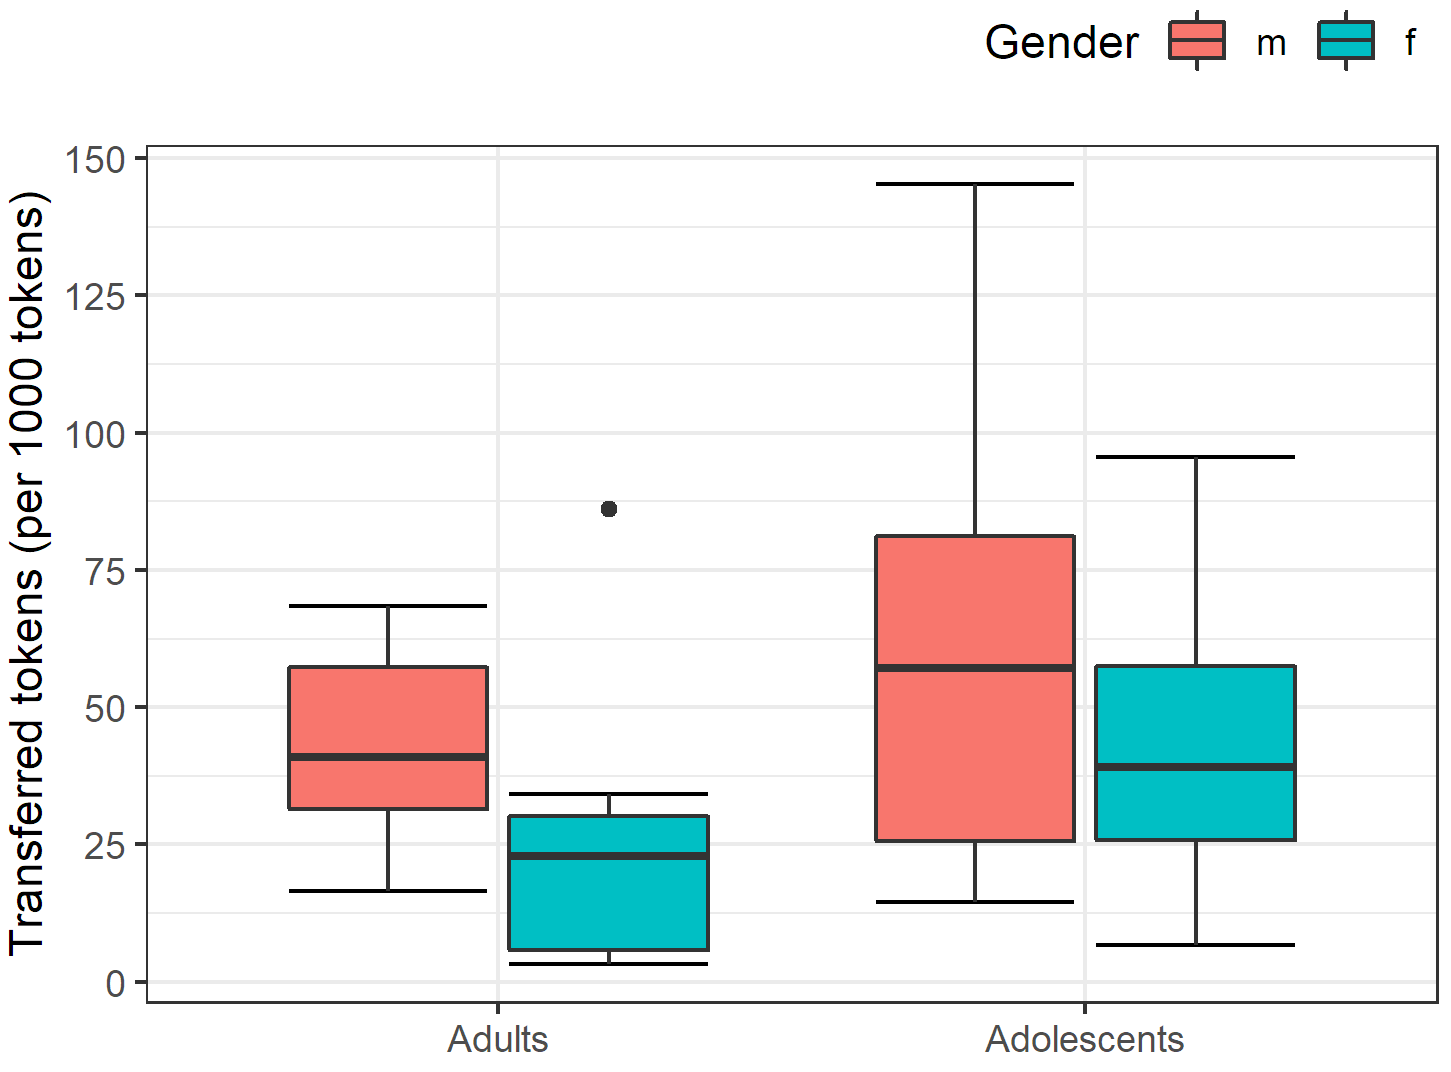
\includegraphics[width=0.8\textwidth]{figures/brackefig1.png}
\caption{Individual relative frequencies of transferred tokens of male and female adults and adolescents\label{fig:bracke:1}}
\end{figure}

Now I turn to the frequency of use of transferred lexical items with respect to speaker gender. The corpus linguistic approach to the data shows that the male subcorpora contain relatively more transferred tokens than the female subcorpora in both age groups. The difference is 17 tokens per 1000 in the case of the adolescents and 22 tokens per 1000 in the case of the adults (see the values in square brackets in Tables~\ref{tab:bracke:4} and~\ref{tab:bracke:5}, respectively). Since the adult subcorpus contains fewer transferred tokens overall, this means that the men’s corpus contains almost twice as many transferred tokens as the women’s corpus.\footnote{Importantly, excluding the three young speakers from Windhoek (two male, one female) from the sample of adults does not change the relative 2:1 ratio of other-language items between men and women. The remaining men use 110 transferred and 3169 other tokens, the remaining women use 136 transferred and 8395 other tokens ($\chi^2 = 35.993; p < 0.001; \varphi = 0.055$).} In both age groups the difference between the male and the female subcorpus is statistically significant according to the χ² test (adolescents: $\chi^2 = 131.587; p < 0.001; \varphi = 0.038$; adults: $\chi^2 = 53.961; p < 0.001; \varphi = 0.061$). The effect size is higher in the case of the adults.

\begin{table}
\begin{floatrow}\captionsetup{margin=.1\textwidth}
\ttabbox[.425\textwidth]{%
\begin{tabular}{lrr}
\lsptoprule
 & \multicolumn{2}{c}{Tokens}\\\cmidrule(lr){2-3}
 & Transferred [rel.] & Other\\
\midrule
Boys & 2190 [60.6] & 33950\\
Girls & 2392 [43.6] & 52466\\
\lspbottomrule
\end{tabular}}
{\caption{Distribution of tokens over boys and girls\label{tab:bracke:4}}}%
\ttabbox[.575\textwidth]{\begin{tabular}{lrr} 
\lsptoprule
 & \multicolumn{2}{c}{Tokens}\\\cmidrule(lr){2-3}
 & Transferred [rel.] & Other\\
 \midrule
Men & 233 [45.2] & 4920\\
Women & 221 [23.2] & 9298\\
\lspbottomrule
\end{tabular}}
{\caption{Distribution of tokens over men and women\label{tab:bracke:5}}}
\end{floatrow}
\end{table}  

So far the data seems to corroborate the assumption that male speakers use more transferred lexical items than female speakers. However, more than in the case of the age groups, the results of the analysis of individual frequencies for the gender groups deviate from the result of the corpus linguistic approach. \figref{fig:bracke:1} displays the individual frequencies of transferred tokens among male and female adults (boxplots on the left) and adolescents (boxplots on the right). It visualizes the dispersion of values between individuals within and among groups. Among the women dispersion is larger than among the men. On the one hand, three women used less than seven transferred lexical items per 1000 tokens, on the other hand the adult speaker who used the most (86.0) is also a woman, namely the young women from Windhoek mentioned above. Dispersion is even higher among adolescents. In this age group, the frequencies of female speakers are slightly more uniform than those of males. The first quartile (the lower border of the boxes in \figref{fig:bracke:1}) lies at just below 26 transferred tokens per 1000 tokens for both boys and girls but the third quartile of the boys lies at 81.1, exceeding the girls’ third quartile by a margin of more than 23. Importantly, these individual results show that substantial differences exist also within the gender groups of each age group. Not all male and not all female speakers behave similar to one another. Furthermore, even though the median is higher by approximately 18 for male speakers in either age group, applying a one-tailed Wilcoxon rank-sum test provides results that are slightly above the significance level of 0.05 (adolescents: $W = 377; p = 0.079$; adults: $W = 37; p = 0.054$). That means, on an individual level, one cannot speak of a significant difference between male and female speakers in the same age group.

Concerning the relationship between speakers of the same gender in different age groups, it can be said that girls and women in the corpus behave less similar to each other than men and boys. In \figref{fig:bracke:1}, this is illustrated by the very small overlap between the boxes for the interquartile range of girls and women and it is reflected in a significant result of a one-tailed rank-sum test ($W = 186; p = 0.025$). The two groups behaving most similar are teenage girls and adult men who have almost identical medians ({\textasciitilde}40) and a similar interquartile range.\largerpage[-1]

The analysis has already demonstrated that the quantity of transferred tokens is not a simple function of a single sociolinguistic variable.  For the adolescents, I explored this further by considering an additional factor, namely the type of school attended by the speakers. I chose this variable (a) because school is the everyday social environment for students and this environment may influence their language use, and (b) because the schools attended by the speakers differ with respect to the role of German in the institution. That is, speakers are subject to different amounts of instruction in German and in other languages. The schools that speakers attended fall into three categories:\footnote{Previous tests for each individual school suggested that students of schools falling into one of these three categories behave more similarly to each other than to students from another group.}

  
\begin{enumerate}   
	\item The school receives funding from the Federal Republic of Germany, several subjects are taught in German: German Foreign School (\textit{Deutsche} \textit{Auslandsschule}, GFS).
  	
	\item The school offers the subject \textit{Deutsch} \textit{als} \textit{Muttersprache} (‘German as a mother language’, DaM), no other subjects are taught in German: DaM school
    
	\item The school does not offer any instruction in German: no-German-school. (Note, all students in the sample who attended this kind of school did, however, take private German lessons.)
 \end{enumerate}

The \textit{Deutsche} \textit{Höhere} \textit{Privatschule} in Windhoek is the only school in Namibia belonging to the first category. Community members widely consider it an important institution for (“good”) German in Namibia. Most students in the sample went to a school in the second category with some instruction in German, while a few students only took private German lessons (see \tabref{tab:bracke:6}). As mentioned earlier, the distribution of participants over gender and school type is not equal.

  

  
\begin{table}  
\begin{tabular}{lrrr}
\lsptoprule
      & \multicolumn{1}{c}{Female} & \multicolumn{1}{c}{Male} & \multicolumn{1}{c}{Total}\\
\midrule
{GFS} & {11} & {6} & {17}\\
{DaM} & {19} & {9} & {28}\\
{No German} & {2} & {4} & {6}\\
\lspbottomrule
\end{tabular}
\caption{Adolescent speakers per category of school\label{tab:bracke:6}}
\end{table}

\begin{figure}
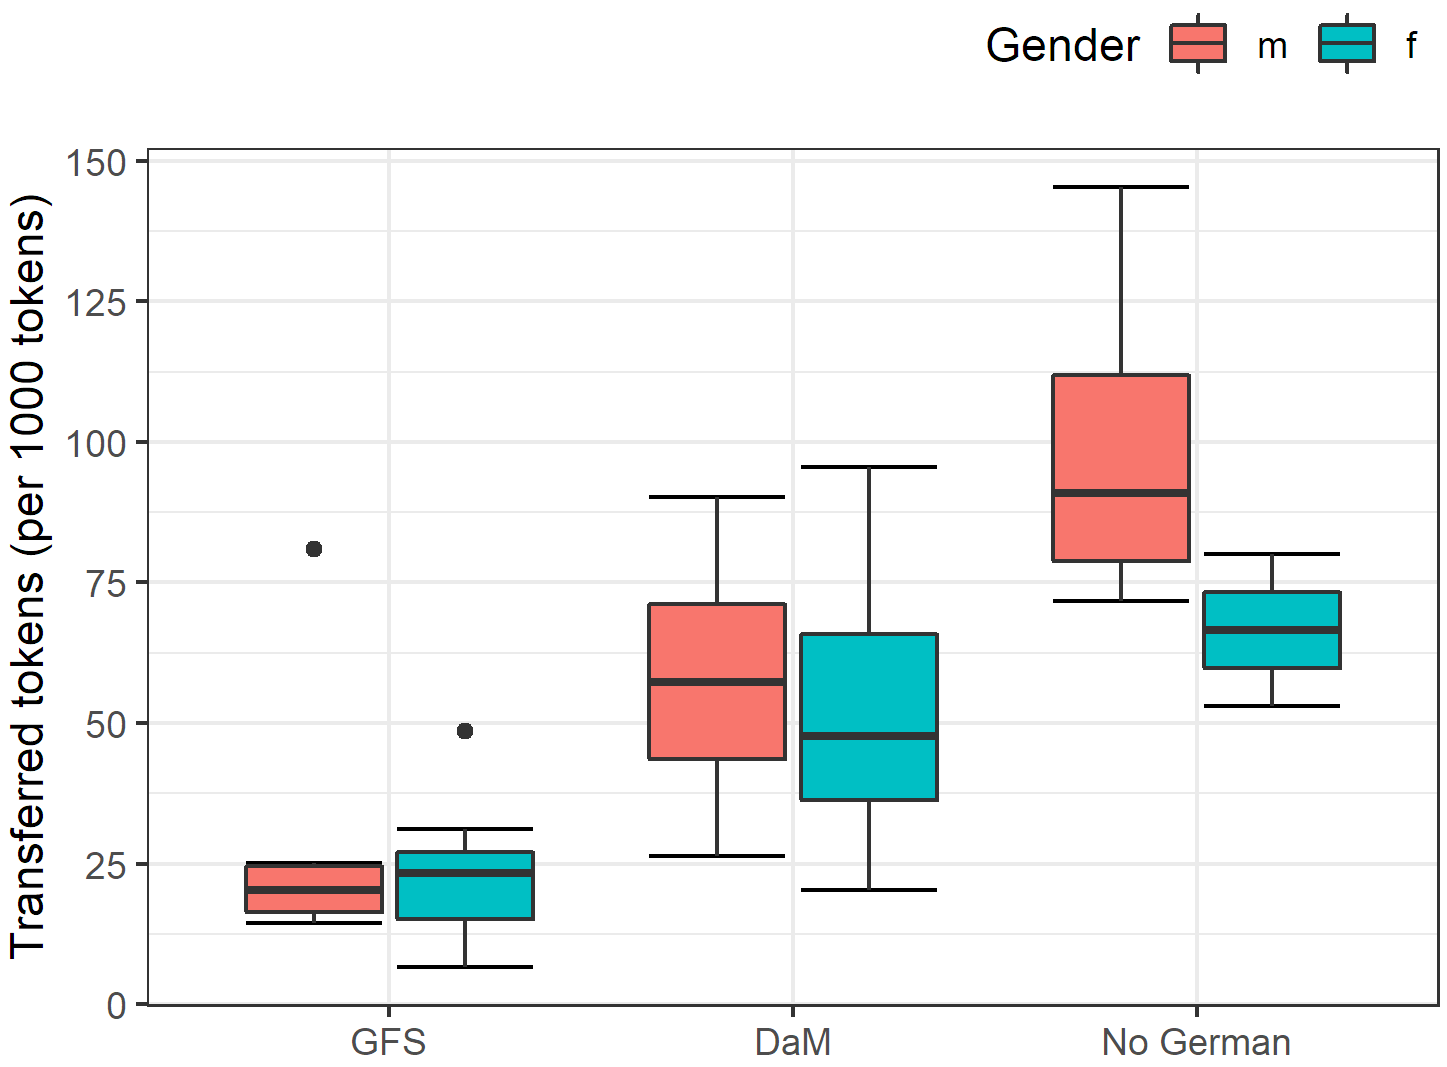
\includegraphics[width=0.8\textwidth]{figures/brackefig2.png}
 \caption{Individual relative frequencies of transferred tokens of male and female adolescents by school category}
 \label{fig:bracke:2}
 \end{figure}

The results of analyzing the individual frequencies\largerpage{} show an interesting pattern (\figref{fig:bracke:2}). There are significant differences between the three groups corresponding quite obviously to the status of German in the school.\footnote{A one-tailed Wilcoxon rank-sum test gives the following results. GFS vs. DaM: $W = 428, p < 0.001$; DaM vs. No German: $W = 141, p = 0.004$.} At the same time, gender differences within groups are not significant. The median differs by less than three tokens per 1000 tokens (girls > boys) for the GFS and by less than ten tokens (boys > girls) for the DaM schools. For students attending schools without German instruction the gender differences are larger, with the boys’ median being higher by a margin of 24. However, it has to be noted that this sample only contains four boys and two girls, which is also why the Wilcoxon rank-sum test could not provide a significant result. By contrast, the corpus linguistic approach does provide a significant difference for this sample ($\chi^2 = 25.054; p < 0.001; \varphi = 0.042$). For the other two school categories the corpus linguistic approaches results are as follows: There is no significant difference between boys and girls from the largest group, the DaM schools ($p = 0.997$). For the GFS school this approach indicates a significant difference ($\chi^2 = 25.431; p < 0.001; \varphi = 0.028$), but as \figref{fig:bracke:2} shows this is due to a single male student who exceeds all of his fellow male students (and most of his fellow female students) by at least 50 transferred tokens per 1000. That is, the data really only suggests a difference between boys and girls in the smallest category, the no-German schools. Note that this school category is also the only one in which there is an overproportional amount of male speakers. That is, the results for all boys and all girls presented above seem to be somewhat skewed by the fact that more than one in five boys in the sample goes to a no-German-school but only one in 16 girls. Therefore, exploring the additional sociolinguistic variable school type revealed that the findings concerning gender differences for adolescents should be treated with caution.
  

Unfortunately, a similar analysis for the adult speakers, which would focus on occupation and workplace, was not possible due to the small sample size of only 14 speakers. An observation suggesting that these aspects might well be relevant is that three women in the sample are school or pre-school teachers and two of them are among the women mentioned above who used very few transferred lexical items.

 
   
\subsection{Proportion of donor languages}
\label{sec:bracke:5.2}

In addition to the frequency analysis of transferred tokens, I investigated how many of the transferred types and tokens are taken from English, Afrikaans and other Namibian languages. The results show that English and Afrikaans are by far the two most important donor languages in the data. 98.6 percent of the 1147 transferred types used by adolescents originate from one of these two languages. In the adult corpus, this applies to all except one of the 210 types. Thus, Bantu and Khoisan languages only play a minor role in the data as compared to the two Germanic languages, which is why I concentrate on the latter in the following. The columns \textit{E} and \textit{A} in \tabref{tab:bracke:7} display the absolute frequencies of English and Afrikaans types and tokens in each of the four speaker groups, the percentages represent the proportion of English vs. Afrikaans types/tokens. These results show that, consistently, English is the dominant donor language in the data. In the corpora of all four speaker groups, the proportion of English types and tokens is higher than that of Afrikaans types and tokens. However, the ratios of English and Afrikaans differ somewhat between groups. English is most dominant in the girls subcorpus, followed by boys, then women and finally men. That is, with respect to all transferred types/tokens, adults used more material of Afrikaans origin than adolescents, and in both age groups male speakers used more material of Afrikaans origin than female speakers, with a larger difference between men and women.\footnote{It is a different question how many Afrikaans-origin transferred tokens are used with respect to all tokens (not only with respect to all transferred tokens as above). This has to do with the fact that adults use fewer transferred tokens overall. That is why women have a lower relative frequency (4.1) of Afrikaans tokens (per 1000 tokens) than girls (5.1) and boys (10.0). Despite the fact that men also use fewer transferred tokens than adolescents, they still have the highest proportion of Afrikaans-origin transferred tokens per 1000 tokens (14.7).} For tokens (but not for types), all of these differences are significant.

  

  
\begin{table}
\begin{tabular}{lrrrrrrrr}
\lsptoprule
& \multicolumn{4}{c}{Types} & \multicolumn{4}{c}{Tokens}\\\cmidrule(lr){2-5}\cmidrule(lr){6-9}
		& \multicolumn{1}{c}{E} & \multicolumn{1}{c}{A} & \multicolumn{1}{c}{\% E} & \multicolumn{1}{c}{\% A} & \multicolumn{1}{c}{E} & \multicolumn{1}{c}{A} & \multicolumn{1}{c}{\% E} & \multicolumn{1}{c}{\% A}\\
\midrule
Boys & 531 & 87 & 85.9 & 14.1 & 1782 & 363 & 83.1 & 16.9\\
Girls & 614 & 81 & 88.4 & 11.7 & 2097 & 278 & 88.3 & 11.7\\
Men & 98 & 37 & 72.6 & 27.4 & 156 & 76 & 67.2 & 32.8\\
Women & 85 & 19 & 81.7 & 18.3 & 178 & 39 & 82.0 & 18.0\\
\lspbottomrule
\end{tabular}
\caption{Absolute frequency and proportion of English and Afrikaans types and tokens\label{tab:bracke:7}}
\end{table}  

The dominance of English partly goes back to the use of dictionary-attested forms. For example, the 452 occurrences of the type \textit{okay} account for almost 9 percent of all transferred tokens. However, as \tabref{tab:bracke:8} displays, non-attested forms make up the majority of English-origin material in all groups. Even if only non-attested English-origin tokens/types are considered, these are still more frequent than Afrikaans-origin types and tokens. \tabref{tab:bracke:8} also shows that, while the ratio of attested to non-attested English-origin types is rather similar across groups, the ratio of attested to non-attested \textit{tokens} differs significantly in both age groups. Girls use about ten percent more attested tokens than boys ($\chi^2 = 47.496; p < 0.001; \varphi = 0.111$) and women about 14 percent more than men ($\chi^2 = 7.317; p = 0.007; \varphi = 0.148$).

  
\begin{table}
\begin{tabular}{lrrrrrrrr}
\lsptoprule
& \multicolumn{4}{c}{Types} & \multicolumn{4}{c}{Tokens}\\\cmidrule(lr){2-5}\cmidrule(lr){6-9}
& \multicolumn{1}{c}{att} & \multicolumn{1}{c}{n-att} & \multicolumn{1}{c}{\% att} & \multicolumn{1}{c}{\% n-att} & \multicolumn{1}{c}{att} & \multicolumn{1}{c}{n-att} & \multicolumn{1}{c}{\% att} & \multicolumn{1}{c}{\% n-att}\\
\midrule
Boys & 139 & 392 & 26.2 & 73.8 & 402 & 1380 & 22.6 & 77.4\\
Girls & 153 & 461 & 24.9 & 75.1 & 682 & 1415 & 32.5 & 67.5\\
Men & 22 & 76 & 22.5 & 77.6 & 46 & 110 & 29.5 & 70.5\\
Women & 24 & 61 & 28.2 & 71.8 & 78 & 100 & 43.8 & 56.2\\
\lspbottomrule
\end{tabular}
\caption{Distribution and proportion of English types and tokens in terms of dictionary attestation (att) or non-attestation (n-att)\label{tab:bracke:8}}
\end{table}  

The overall tendency concerning the differences between male and female speakers with respect to the proportion of English and Afrikaans words is somehow reflected in the use of the most frequent Afrikaans-origin type, \textit{net.} The word meaning ‘just’ or ‘only’, as in \REF{ex:bracke:8}, occurs 199 times as a transferred token in the entire corpus.

\ea
\label{ex:bracke:8}
\gll wir wolltn \textbf{net} essn gehn normal un das war so fancy\\
     we.\textsc{nom} want.\textsc{3pl.pret} just eat.\textsc{inf} go.\textsc{inf} normally and that be.\textsc{3sg.pret} so fancy\\
\glt `We just wanted to go out for an ordinary dinner and that was so fancy.' {[}NAM092W1{]}
\z

The relative frequency of \textit{net} among male speakers is about twice as high as among female speakers in either age group. Importantly, \textit{net} is also more frequent among male speakers relative to the Standard German alternatives \textit{nur} and \textit{bloß.} This can be shown by dividing the token counts for \textit{net} by the sum of the token counts of all three words with similar meaning. The resulting proportion of \textit{net} is 45.3 percent for boys and 30.4 percent for girls, 33.3 percent for men and 16.4 percent for women. The type is also more widespread among male speakers: Four out of six men and 17 out of 19 boys used it (89.5\%), while only half of the eight women and 19 out of 32 girls (59.4\%) used \textit{net} at least once.

Much more could be said about the use of individual lexical items by different speakers. However, since this chapter has limited space, I now come to its final section for a summary and discussion.

 
\section{Summary and discussion}
\label{sec:bracke:6}
 

Concerning the key aspect of the study, the quantity of transferred lexical items (other-language tokens, excluding instances of multi-word CS) in free conversations, the most obvious finding is that the phenomenon is ubiquitous in informal Namibian German. To some extent all speakers used transferred words, although the quantity varied substantially between individuals. Due to the perception of mixed and unmixed language in the NG community, a high frequency of transferred lexical items can be interpreted as a stronger deviation from the standard than a low frequency. The assumption that young speakers use more transferred lexical items than older speakers was generally supported by the data analysis. The results for the adults indicated that a more fine-grained analysis of language use by age would be desirable if the size of the data set allowed it. The results concerning the assumption that male speakers used more transferred words than female speakers were less clear. The analysis suggests that the assumption is not true independent of other sociolinguistic variables. This became apparent by looking at gender and age, as well as at gender and school. For gender and age it was observed that, overall, teenage girls behaved rather similar to the group of adult men, while boys used the most and women the least relative amount of transferred tokens. Thus, within both age groups, male speakers used more transferred lexical items. However, whether this constitutes a significant difference depends on the statistical approach to the data. As opposed to age differences, gender differences were only significant with the broader corpus linguistic approach. Substantial intra-group differences were the reason for this. Furthermore, the analysis for gender and school indicated that gender differences in the group of adolescents may be an artifact of the sample composition. I observed that there are no significant gender differences for speakers of the DaM schools and that differences at the GFS go back to a single student. The differences are larger for speakers attending a school without instruction in German, with boys using more transferred lexical items than girls, but this subsample is also the smallest. Importantly, it was observed that, independent of gender, students who go to different types of schools (concerning the role of German) behave quite differently from one another. Students from the prestigious GFS, who receive the highest amount of German-language instruction, stood out as generally using very few transferred lexical items, while students with no subjects in German used the most. As the latter is the only group with more boys than girls the overall results for boys and girls are somewhat skewed in the direction that boys use more transferred tokens. Generally, this underlines the importance of a sophisticated quantitative analysis that takes into account different metadata and individual speaker behavior. The findings for the schools are also important in and of themselves. They strongly suggest that the frequency with which a speaker uses languages other than German in their everyday life influences their use of transferred lexical items. Moreover, since the schools have different reputations and orientations, the school a student attends likely says something about how important (Standard) German is for their parents. That is, these students are presumably confronted with different language ideologies in their home too, which they might have adopted.

In addition to the general frequency of transferred tokens, the role of donor languages was investigated. In the corpus data, English turned out to dominate quantitatively as a donor language, followed by Afrikaans, while other Namibian languages played only a minor role. The finding that English is more influential than Afrikaans is particularly noteworthy since it is at variance with previous accounts of the role of donor languages in Namibian German, including the recent quantitative analysis by \citet{zimmer_linguisticvar_toappear}. A reason for this may lie in the different data Zimmer and I used. Zimmer’s study is based on Namibian German translations of “Wenker sentences”, that is, on productions that are less spontaneous than informal conversations and might be subject to stylization.\footnote{Cf. also \citegen[116]{radke_lekker_2017} finding that the most frequent transferred items in highly stylized newspaper commentaries in the German-language Namibian newspaper \textit{Allgemeine} \textit{Zeitung} are predominantly of Afrikaans origin.} Concerning the dominance of Afrikaans loanwords across all age groups in his data, \citet{zimmer_linguisticvar_toappear} himself suggests that this could be “an artefact of the design: maybe Afrikaans words are considered particularly salient and are used in the translations to emphasise the deviance of Namdeutsch from European German”. This assumption is corroborated by several interview statements from community members in the \textit{DNam} corpus. When asked about vocabulary they perceive as typical for NG, speakers predominantly mentioned terms originating from Afrikaans, such as \textit{braaien} (see \sectref{sec:bracke:2}), \textit{net} (see \sectref{sec:bracke:5.2}), \textit{mooi} (see example \ref{ex:bracke:3}), \textit{pad} (‘road’), \textit{lekker} (in the sense of ‘good’/‘pleasant’). Yet, spontaneous language in the \textit{DNam} corpus turned out to be influenced by English to a much larger extent than by Afrikaans. An explanation for this apparent mismatch might be that words from Afrikaans are more salient because they are older, since Afrikaans was more important than English until Namibian independence in 1990. Speakers may still know many Afrikaans words because these used to be more common in the past, therefore perceive them as salient, and accordingly put them to use in translations of “Wenker sentences”. At the same time, Afrikaans words might be declining in actual NG language use, which would explain the results of this study. This might also explain the fact that younger speakers used even fewer transferred words from Afrikaans than older speakers in their informal conversations. It would not, however, account for the differences between male and female speakers in both age groups. Still, the salience of Afrikaans might play a role here as well. Afrikaans words are perceived as indexical of a traditional Namibian German identity, which, as I have argued above, seems to have connotations of stereotypical masculinity. Therefore, sounding “typically Namibian” might overlap with sounding “typically male” and speakers who seek to construct a traditional male identity might do so by using features also indexical of a traditional Namibian German identity. By contrast, English is presumably rather associated with modern Namibia and a globalized, English-speaking world. Thus, for speakers orienting themselves away from traditional views and structures in the community, English might be more attractive. This could be a reason why young female community members are particularly inclined towards English-origin lexical material.\footnote{It was also observed that female speakers use significantly more dictionary-attested English-origin tokens than male speakers in the same age group. That is, in this respect the speech of female speakers appears to be closer to the prestige variety Standard German.} It would be necessary to further investigate these hypotheses and the assumptions I made. One could, for example, study the community attitudes towards English and Afrikaans on the one hand and towards (traditional) gender roles on the other and explore whether these attitudes are reflected in speakers’ language use. This study has indicated that there might be an interesting sociolinguistic dynamic at work.

Although I have focused on the aspects of gender and age, this study has also indicated that these are not the only aspects that play a role for the use of transferred lexical items in NG. The findings concerning schools suggest that everyday language use is of importance. This also raises the question of differences between urban and rural dwellers because Namibian German farmers often speak Afrikaans with black farm laborers and with farmers belonging to the Afrikaans-speaking community, whereas in cities English prevails as the language of business. Aside from the place of work and living, language use with family and friends is certainly another aspect to focus on in future studies. The role and interaction of various sociolinguistic variables such as those discussed here in the use of transferred lexical items could further be investigated using a multifactorial statistical model.

I will conclude this chapter with some remarks concerning its methodological aspects. I think, with this study, I have made a case for a careful approach to corpus data. When studying a phenomenon in a corpus that contains productions by a number of speakers, researchers should not only look at aggregated totals but also at the individual behavior of all speakers. Only then it is possible to assess how widespread the phenomenon in question is and how strongly its occurrence varies within the corpus (cf. \citealt{gries_useful_2010}: 274). Lastly, as a prerequisite for the analysis, I have presented my approach to categorizing other-language material in the corpus with the help of a simple annotation system. Note again that the results presented in this chapter concern a subset of the other-language material in the corpus selected on the basis of that annotation, excluding all tokens treated as multi-word code-switches. Certainly, studies based on different selections of other-language data are conceivable. As the annotations will be available for users of the \textit{DNam} corpus in the future, it will be possible for researchers interested in language mixing phenomena in NG to choose their own set of other-language data. I hope that this chapter has helped to stimulate interest in such further research and look forward to its results.

\section*{Acknowledgements}
This chapter is based on my master thesis which I wrote within the project “Namdeutsch: Die Dynamik des Deutschen im mehrsprachigen Kontext Namibias”. I was a part of this project as a student assistant and research assistant, contributing to the creation of the corpus \textit{Deutsch} \textit{in} \textit{Namibia} (\textit{DNam}). The project was funded by the Deutsche Forschungsgemeinschaft (DFG, ‘German Research Foundation’) – WI 2155/9-1; SI 750/4-1. I thank the editor of this volume, Heike Wiese, Pia Schlickeiser, and the anonymous reviewers for helpful comments on earlier versions of this chapter.

{\sloppy\printbibliography[heading=subbibliography,notkeyword=this]}
\end{document} 
